%!TEX root = thesis.tex
\chapter{\code{FASMA} and machine learning}
\label{cha:fasmaML}

With the increasing amount of astrophysical data, it is important to perform a rapid and trustworthy
analysis. This is one of the strengths for \code{FASMA} when dealing with high quality spectroscopic
data for determination of stellar atmospheric parameters. Here a classic method to analyse these
large amount of data has been modernised with a new minimisation technique that utilise the physical
knowledge about the system. However smart it may sound like, it can be improved. The time consuming
part in \code{FASMA} are the calls to \code{MOOG}. In the end a couple of minutes are spent on the
minimisation on a modern computer.

This lead to a side-project: explorer the use of machine learning to determine stellar atmospheric
parameters. Machine learning (ML) is not a new topic in computer science, but it is a tool that is
steadily becoming more and more popular in today's science. The effort of using ML here is meant as
a proof of concept, and something that can be improved upon in the future.

The idea was to remove the expensive calls to \code{MOOG} completely. Two things are required in
order to do so in the approach presented here:
\begin{enumerate}
  \item Stellar atmospheric parameters of a large sample of stars with a big span in the parameter
        space
  \item The EW measurements of as many absorption lines as possible (in this case \ion{Fe}{I} and
        \ion{Fe}{II})
\end{enumerate}
Additionally it is here required that the above two points are obtained in a homogeneous way.
Luckily such a sample was already analysed during this thesis as a test of \code{FASMA} (see
\sref{sec:fasma_test}) where a sample of 582 stars were analysed; all of which meet the above
required criteria.

This data set of measurements of EWs and the parameters were organised and prepared in a big table
as follows:
\begin{itemize}
  \item Each row contains both the measurements of the EWs (first N columns) and the parameters
        (last four columns). The parameters are $T_\mathrm{eff}$, $\log g$, $[\ion{Fe}/\ion{H}]$,
        and $\xi_\mathrm{micro}$
  \item The columns excluding the last four are labelled with the wavelength of the absorption line
  \item All wavelength columns which contained at least one missing measurement of the EW for any
        of the 582 stars were removed
\end{itemize}
There are 58 wavelength columns after removing wavelength columns with missing measurements. Before
the removal there were 299 columns with wavelength. In this case the \code{scikit-learn}
package\footnote{\url{http://scikit-learn.org/}} from the Python ecosystem was used to train the
data set. This also package also include a tool to split the data into a training part and testing
part. This is particular useful when trying to evaluate the accuracy of the model used. Here the
training consist of 2/3 of the data, and the rest is for testing. This splitting is done randomly,
giving slight different results each time the script is executed.

The training itself is quite fast (less than \SI{10}{s}). However, the real power comes when the
trained model is saved to the disk, which can later be loaded again. In this way the training will
only be done once. Using the model to obtain the parameters is much less than \SI{1}{s}, which makes
is many orders of magnitudes faster\footnote{Improvements in the order of millions have been
obtained here.} than a more traditional approach as with \code{FASMA}.

When testing the model trained, the 1/3 data set is used to derive parameters. Those derived
parameters are then compared to the actual parameters with a mean absolute error. This gives an idea
of the accuracy. In \fref{fig:ml} the script was run 1000 times (the splitting was done randomly in
each run), and the error for each parameter is shown as a histogram. The mean errors for each
parameters are roughly $T_\mathrm{eff}:\SI{47}{K}$, $\log g:\SI{0.10}{dex}$,
$[\ion{Fe}/\ion{H}]:\SI{0.038}{dex}$, and $\xi_\mathrm{micro}:\SI{0.12}{km/s}$.

\begin{figure}[htpb!]
    \centering
    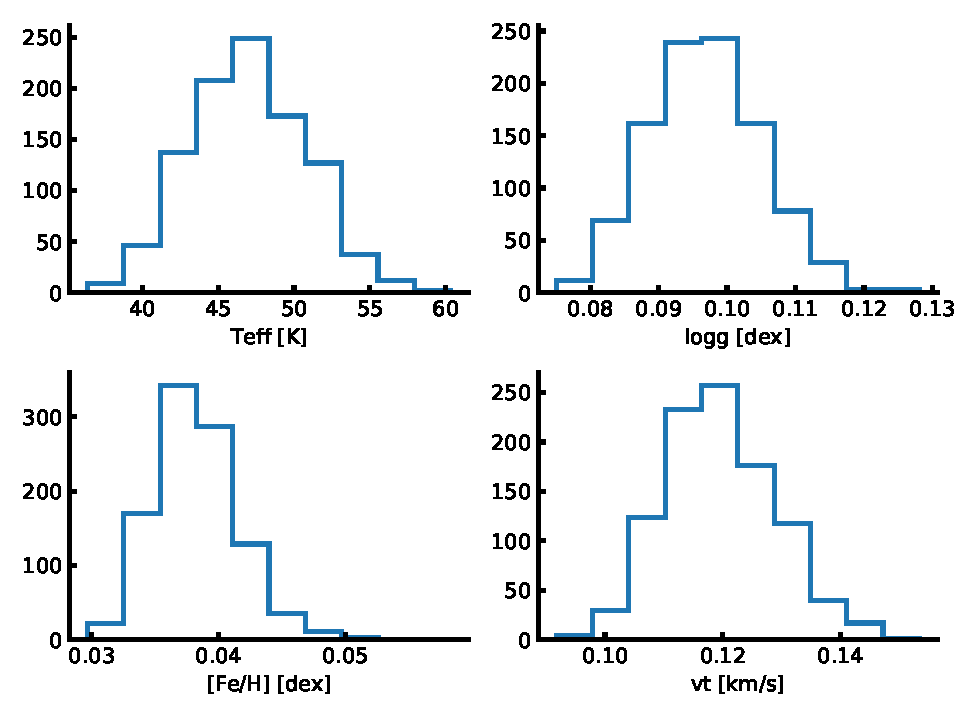
\includegraphics[width=1.0\linewidth]{figures/ML.pdf}
    \caption{Mean absolute error on each parameter after 1000 runs.}
    \label{fig:ml}
\end{figure}

There exists many different algorithms within \code{scikit-learn} to train the final model. In the
test here a simple \code{LinearRegression} was used. Other algorithms were tested as well, such as
\code{Ridge} and \code{Lasso}, however with very similar results. The main difference between the
different algorithms lies in the details on how the minimisation is done. This is described in great
detail in the online documentation.
